%=====================================================================
%  Experimental and DFT-Assisted Raman Characterisation of
%  Isolated N-Acetylmuramic Acid
%
%  Sukesh P, Indian Institute of Technology Jodhpur
%
%  Compile:  pdflatex -> bibtex -> pdflatex -> pdflatex
%  Target:   Spectrochimica Acta A / Vibrational Spectroscopy
%
%  NOTE: values marked  <<CHECK>>  must be verified by the author
%        before submission.
%=====================================================================
\documentclass[preprint,12pt]{elsarticle}

\usepackage{amsmath,amssymb}
\usepackage{graphicx}
\usepackage{booktabs}
\usepackage{longtable}
\usepackage[version=4]{mhchem}
\usepackage{siunitx}
\usepackage{textgreek}
\usepackage{lineno}
\usepackage[hidelinks]{hyperref}

\journal{Spectrochimica Acta Part A: Molecular and Biomolecular Spectroscopy}

\newcommand{\wn}{\ensuremath{\mathrm{cm}^{-1}}}
\usepackage{xcolor}
\newcommand{\authorcheck}[1]{\textcolor{red}{[#1]}}

\begin{document}

\begin{frontmatter}

\title{Experimental and DFT-Assisted Raman Characterisation of Isolated
N-Acetylmuramic Acid: Vibrational Assignment and a Reference Spectrum for
Bacterial Cell-Wall Analysis}

\author[iitj]{Sukesh P\corref{cor1}}
\ead{sukeshperiyasamy@gmail.com}
\cortext[cor1]{Corresponding author.}

% \author[iitj]{Supervisor Name}

\affiliation[iitj]{organization={Department of Electrical Engineering,
Indian Institute of Technology Jodhpur},
city={Jodhpur}, postcode={342030}, state={Rajasthan}, country={India}}

\begin{abstract}
N-acetylmuramic acid (MurNAc, NAM) is the defining amino sugar of bacterial
peptidoglycan and underlies many of the vibrational features exploited in
Raman-based microbial identification. Despite this, an experimentally
benchmarked vibrational assignment for the isolated molecule has not been
reported; existing assignments derive either from empirical force-field
treatments of the crystalline hydrate or from density functional theory (DFT)
calculations validated only indirectly against whole-cell bacterial spectra.
Here we report the Raman spectrum of isolated N-acetylmuramic acid
powder, acquired at 785~nm across a systematic grid of 80 acquisition
conditions (five integration times, sixteen laser power levels), together with
harmonic Raman frequencies computed at the B3LYP-D3BJ/6-311++G(d,p) level. Forty-one
reproducible bands were identified in the 400--1800~\wn{} fingerprint region,
of which thirty-three were matched to calculated normal modes with a mean
absolute deviation of 9.1~\wn{}, a root-mean-square deviation of 10.2~\wn{},
and a correlation coefficient of 0.9997. Normal-mode decomposition permitted
assignment of the pyranose ring, glycosidic, lactyl, acetamido and carboxyl
contributions. Notably, the calculated mode falling in the disputed
$\sim$730~\wn{} bacterial marker region is shown to originate almost entirely
from out-of-plane deformation of the carboxylic acid hydroxyl group
(48\% of the mode displacement), with negligible pyranose ring character
(0.5\%). Because this proton is absent in intact peptidoglycan, where the
NAM carboxyl is amide-linked to the peptide stem, the result argues against
attributing the bacterial 730~\wn{} band to muramic acid. The reference
spectrum and assignments reported here provide a validated basis for
interpreting peptidoglycan contributions in bacterial Raman and
surface-enhanced Raman spectra.
\end{abstract}

\begin{keyword}
Raman spectroscopy \sep density functional theory \sep N-acetylmuramic acid \sep
peptidoglycan \sep vibrational assignment \sep bacterial biomarker
\end{keyword}

\end{frontmatter}

\linenumbers

%=====================================================================
\section{Introduction}
%=====================================================================

Raman spectroscopy provides label-free, non-destructive vibrational
fingerprints of biological material and requires minimal sample preparation,
which has made it attractive for rapid microbial characterisation
\cite{wang2022bacteria,ma2024ecoli}. Bacterial Raman spectra are, however,
superpositions of contributions from proteins, nucleic acids, lipids and the
cell wall, and the interpretation of individual bands therefore depends on the
availability of reliable reference spectra for the constituent molecules.

Among cell-wall components, N-acetylmuramic acid occupies a distinctive
position. Together with N-acetylglucosamine (GlcNAc, NAG) it forms the
alternating glycan backbone of peptidoglycan, the polymer that confers
mechanical rigidity on the bacterial cell wall in both Gram-positive and
Gram-negative organisms \cite{vollmer2008}. Unlike GlcNAc, which also occurs widely in
eukaryotic glycans, muramic acid is essentially restricted to bacteria, and
its D-lactyl ether substituent at C-3 is chemically unique to the bacterial
cell wall. This specificity has made NAM an attractive target for
Raman-based and surface-enhanced Raman (SERS) approaches to bacterial
detection.

Raman spectra of structurally related amino sugars have been reported
\cite{she1974raman}, and computational treatments of saccharide Raman spectra
are well established \cite{kaminsky2020saccharides}.
Vibrational studies of muramic acid itself nevertheless remain sparse. Early work
combined infrared and Raman measurements on the crystalline monohydrate with
harmonic dynamics based on empirical force fields \cite{kouach1994}, achieving
an average agreement of approximately 4~\wn{} between observed and calculated
frequencies. More recently, Ma et~al.\ \cite{ma2024ecoli} computed Raman
spectra of NAM and NAG by DFT at the B3LYP/6-311++G(d,p) level in order to
construct a diagnostic model for \emph{Escherichia coli}. In that work,
however, NAM entered only as an \emph{in silico} spectral component: the
calculated spectrum was compared against whole-cell bacterial measurements,
in which peptidoglycan bands are superimposed on strong protein, lipid and
nucleic acid signals. The NAM assignments were therefore never validated
directly.

A further open question concerns the band near 730~\wn{}, one of the
strongest and most frequently used features in bacterial SERS spectra. Its
origin has been variously attributed to adenine and related nucleotide
degradation products \cite{premasiri2016origins,kubryk2016origin} and, less
frequently, to cell-wall components. In the absence of a measured spectrum
of isolated muramic acid, the peptidoglycan contribution to this band could
not be assessed directly.

The present work addresses these gaps. We report the Raman spectrum of
isolated N-acetylmuramic acid powder measured under systematically
optimised acquisition conditions, together with harmonic Raman frequencies
computed by DFT, and we use normal-mode decomposition to assign the observed
bands. The resulting reference spectrum is intended to support the
interpretation of peptidoglycan features in bacterial Raman and SERS
measurements.

%=====================================================================
\section{Materials and methods}
%=====================================================================

\subsection{Materials}

N-acetylmuramic acid (Sigma-Aldrich A3007; CAS 10597-89-4; synthetic;
$\geq$98\% by TLC; white powder; stated residual methanol $\leq$1~mol/mol;
lot \authorcheck{insert lot number from the bottle}) was used as received
without further purification or recrystallisation. The stated molecular weight
of 293.27 corresponds to anhydrous C$_{11}$H$_{19}$NO$_8$; the material is
therefore not a hydrate.

The supplier specification defines five stereocentres but leaves the anomeric
configuration unspecified (SMILES
\texttt{CC(O[C@H]1[C@H](O)[C@@H](CO)OC(O)[C@@H]1NC(C)=O)C(O)=O};
InChI stereo layer \texttt{/t5-,7+,8-,9-,10-/m1/s1}). The material is thus an
anomeric mixture rather than a single anomer, as is usual for a reducing sugar.
This is relevant to the interpretation of the 820--980~\wn{} region and is
discussed in Section~\ref{sec:anomer}.

For measurement, a small quantity of powder was deposited directly onto a clean
glass microscope slide. Samples were handled under ambient laboratory
conditions, and exposure to atmospheric moisture was minimised during
preparation and measurement. The reagent was stored at 2--8~$^\circ$C as
supplied.

\subsection{Raman measurements}

Raman spectra were recorded on a B\&W Tek i-Raman Plus system (model
BWS465-785H) coupled to a BAC102-785E Raman microscope. Excitation was provided
by a 785~nm diode laser (nominal maximum output 495~mW, Class 3B) with an
emission wavelength of 784.92~nm as reported by the instrument software.
Spectra were collected on a 2048-pixel detector spanning $-46$ to
$2842$~\wn{}, of which the 400--1800~\wn{} fingerprint region was retained for
analysis. Spectral sampling varies across the range, from 1.76~\wn{} per pixel
at 400~\wn{} to 1.43~\wn{} per pixel at 1800~\wn{}. Measurements were made through a
20$\times$ Plan objective. Each recorded spectrum was the average of two
successive detector readings.

Acquisition conditions were optimised systematically rather than chosen
\emph{a priori}. A full factorial grid was measured comprising five integration
times (5, 10, 15, 20 and 25~s) and sixteen laser power settings (5--80\% of
nominal output in 5\% steps, corresponding to approximately 25--396~mW of laser
output), giving 80 distinct conditions; additional measurements at 15~s extended
the replicate coverage. In total 98 independent spectra of NAM powder were
acquired. Detector saturation was not observed at any condition. A dark
spectrum was recorded and subtracted by the instrument software for every
measurement.

Laser power incident on the sample was measured directly with a power meter
placed at the objective focal plane and was \authorcheck{XX} mW at the
\authorcheck{YY}\% setting used for the final measurements, corresponding to a
power density of approximately \authorcheck{ZZ} mW\,$\mu$m$^{-2}$ for the
20$\times$ objective. \authorcheck{Insert measured values. Also state the
instrument spectral resolution in \wn{} from the manufacturer specification.}

\subsection{Spectral preprocessing}

All spectra were processed through an identical pipeline. Dark-subtracted
intensities were interpolated onto a uniform 1~\wn{} grid spanning
400--1800~\wn{}. Baseline contributions arising from the substrate and from
residual fluorescence were removed by asymmetric least-squares (ALS) fitting \cite{eilers2005}
with smoothing parameter $\lambda = 10^{5}$, asymmetry $p = 0.001$ and ten
iterations. Baseline-corrected spectra were smoothed with a
Savitzky--Golay filter \cite{savitzky1964} (window 11 points, third-order
polynomial), chosen to
suppress detector noise without measurable distortion of band positions or
widths, and finally min--max normalised.

Signal-to-noise ratio was estimated for each spectrum as the ratio of the
maximum band intensity above the median to the noise standard deviation
determined from successive differences in the signal-free region above
1750~\wn{}. Spectra with SNR $\geq 100$ ($n = 40$) were retained to construct the reference
spectrum. Band positions were located by prominence-based peak detection on the
averaged spectrum.

Distinguishing genuine weak bands from correlated processing artefacts requires
care: baseline correction and smoothing generate reproducible residual
structure, so a band appearing consistently across spectra is not by itself
evidence that it is real. Each candidate band was therefore evaluated against
the local noise level, estimated from successive differences of the averaged
spectrum within a $\pm 50$~\wn{} window. Two independent criteria were applied:
the peak prominence, and the peak height above the local median, each required
to exceed three times the local noise. Bands satisfying both criteria are
reported as high confidence; those satisfying only one are reported but flagged
as tentative; those satisfying neither were discarded. Five candidate features,
at 411, 428, 901, 1495 and 1677~\wn{}, failed both criteria and are not
reported. A reproducibility value is also quoted for each band, defined as the
fraction of the 40 individual spectra in which a peak was independently detected
within $\pm 4$~\wn{} of the mean position.

All processing was performed in Python using NumPy, SciPy and pandas.

\subsection{DFT calculations}

Geometry optimisation and harmonic vibrational frequency calculations were
performed with Gaussian~16 \cite{gaussian16} at the B3LYP level
\cite{becke1993,lee1988} using the 6-311++G(d,p) basis set, with Grimme's D3
dispersion correction and Becke--Johnson damping \cite{grimme2011} and Raman
activities requested. Optimisation used tight convergence criteria with
analytically computed initial force constants, an ultrafine integration grid,
and tight SCF convergence with quadratic convergence enabled
(\texttt{opt=(calcfc,tight) freq=raman int=ultrafine scf=(tight,xqc)}).
Calculations were carried out on the isolated molecule in the gas phase; no
implicit solvation model was applied.

The starting geometry was the $\beta$ anomer of N-acetylmuramic acid. The
optimisation converged to a stationary point and the job reached normal
termination. The optimised structure comprises 39 atoms
(C$_{11}$H$_{19}$NO$_8$) and yielded 111 normal modes, none of which was
imaginary, confirming that the geometry corresponds to a true minimum on the
potential energy surface. As noted in Section~2.1 the measured material is an
anomeric mixture; the calculation therefore models only one component of the
sample, a limitation examined in Section~\ref{sec:anomer}.

Harmonic wavenumbers were scaled by 0.980 below 1800~\wn{} and 0.967 above,
following the scheme applied by Ma et~al.\ \cite{ma2024ecoli}, which permits
direct comparison with the only other modern DFT treatment of this molecule.

Simulated Raman intensities were obtained from the computed Raman activities
$S_i$ using the standard Placzek expression,
\begin{equation}
I_i \;\propto\; \frac{(\nu_0-\nu_i)^4\,S_i}
{\nu_i\left[1-\exp\!\left(-hc\nu_i/k_BT\right)\right]},
\end{equation}
with $\nu_0$ the excitation wavenumber corresponding to 785~nm and
$T = 298.15$~K. The resulting stick spectrum was convolved with Lorentzian
line shapes of 10~\wn{} full width at half maximum for comparison with
experiment.

Mode characters were determined from the calculated Cartesian displacement
vectors. Bond connectivity was established from interatomic distances using
covalent radii, and for each normal mode the fractional contribution of each
atom, of the pyranose ring, and of individual bond stretching coordinates was
evaluated from the mass-weighted displacements. This procedure provides a
quantitative, reproducible basis for the assignments in
Table~\ref{tab:comparison}; it is not equivalent to a full potential energy
distribution analysis, and the principal assignments should be confirmed by
visual inspection of the normal-mode animations.

%=====================================================================
\section{Results and discussion}
%=====================================================================

\subsection{Optimised molecular geometry}

The DFT-optimised structure of $\beta$-N-acetylmuramic acid is shown in
Figure~\ref{fig:structure}. The pyranose ring adopts the expected $^4C_1$
chair conformation, with the acetamido group at C-2, the D-lactyl ether at
C-3 and the hydroxymethyl group at C-5. All 111 computed frequencies are
real, confirming a true minimum on the potential energy surface. Optimised
Cartesian coordinates are given in the Supplementary Material.

\begin{figure}[htbp]
\centering
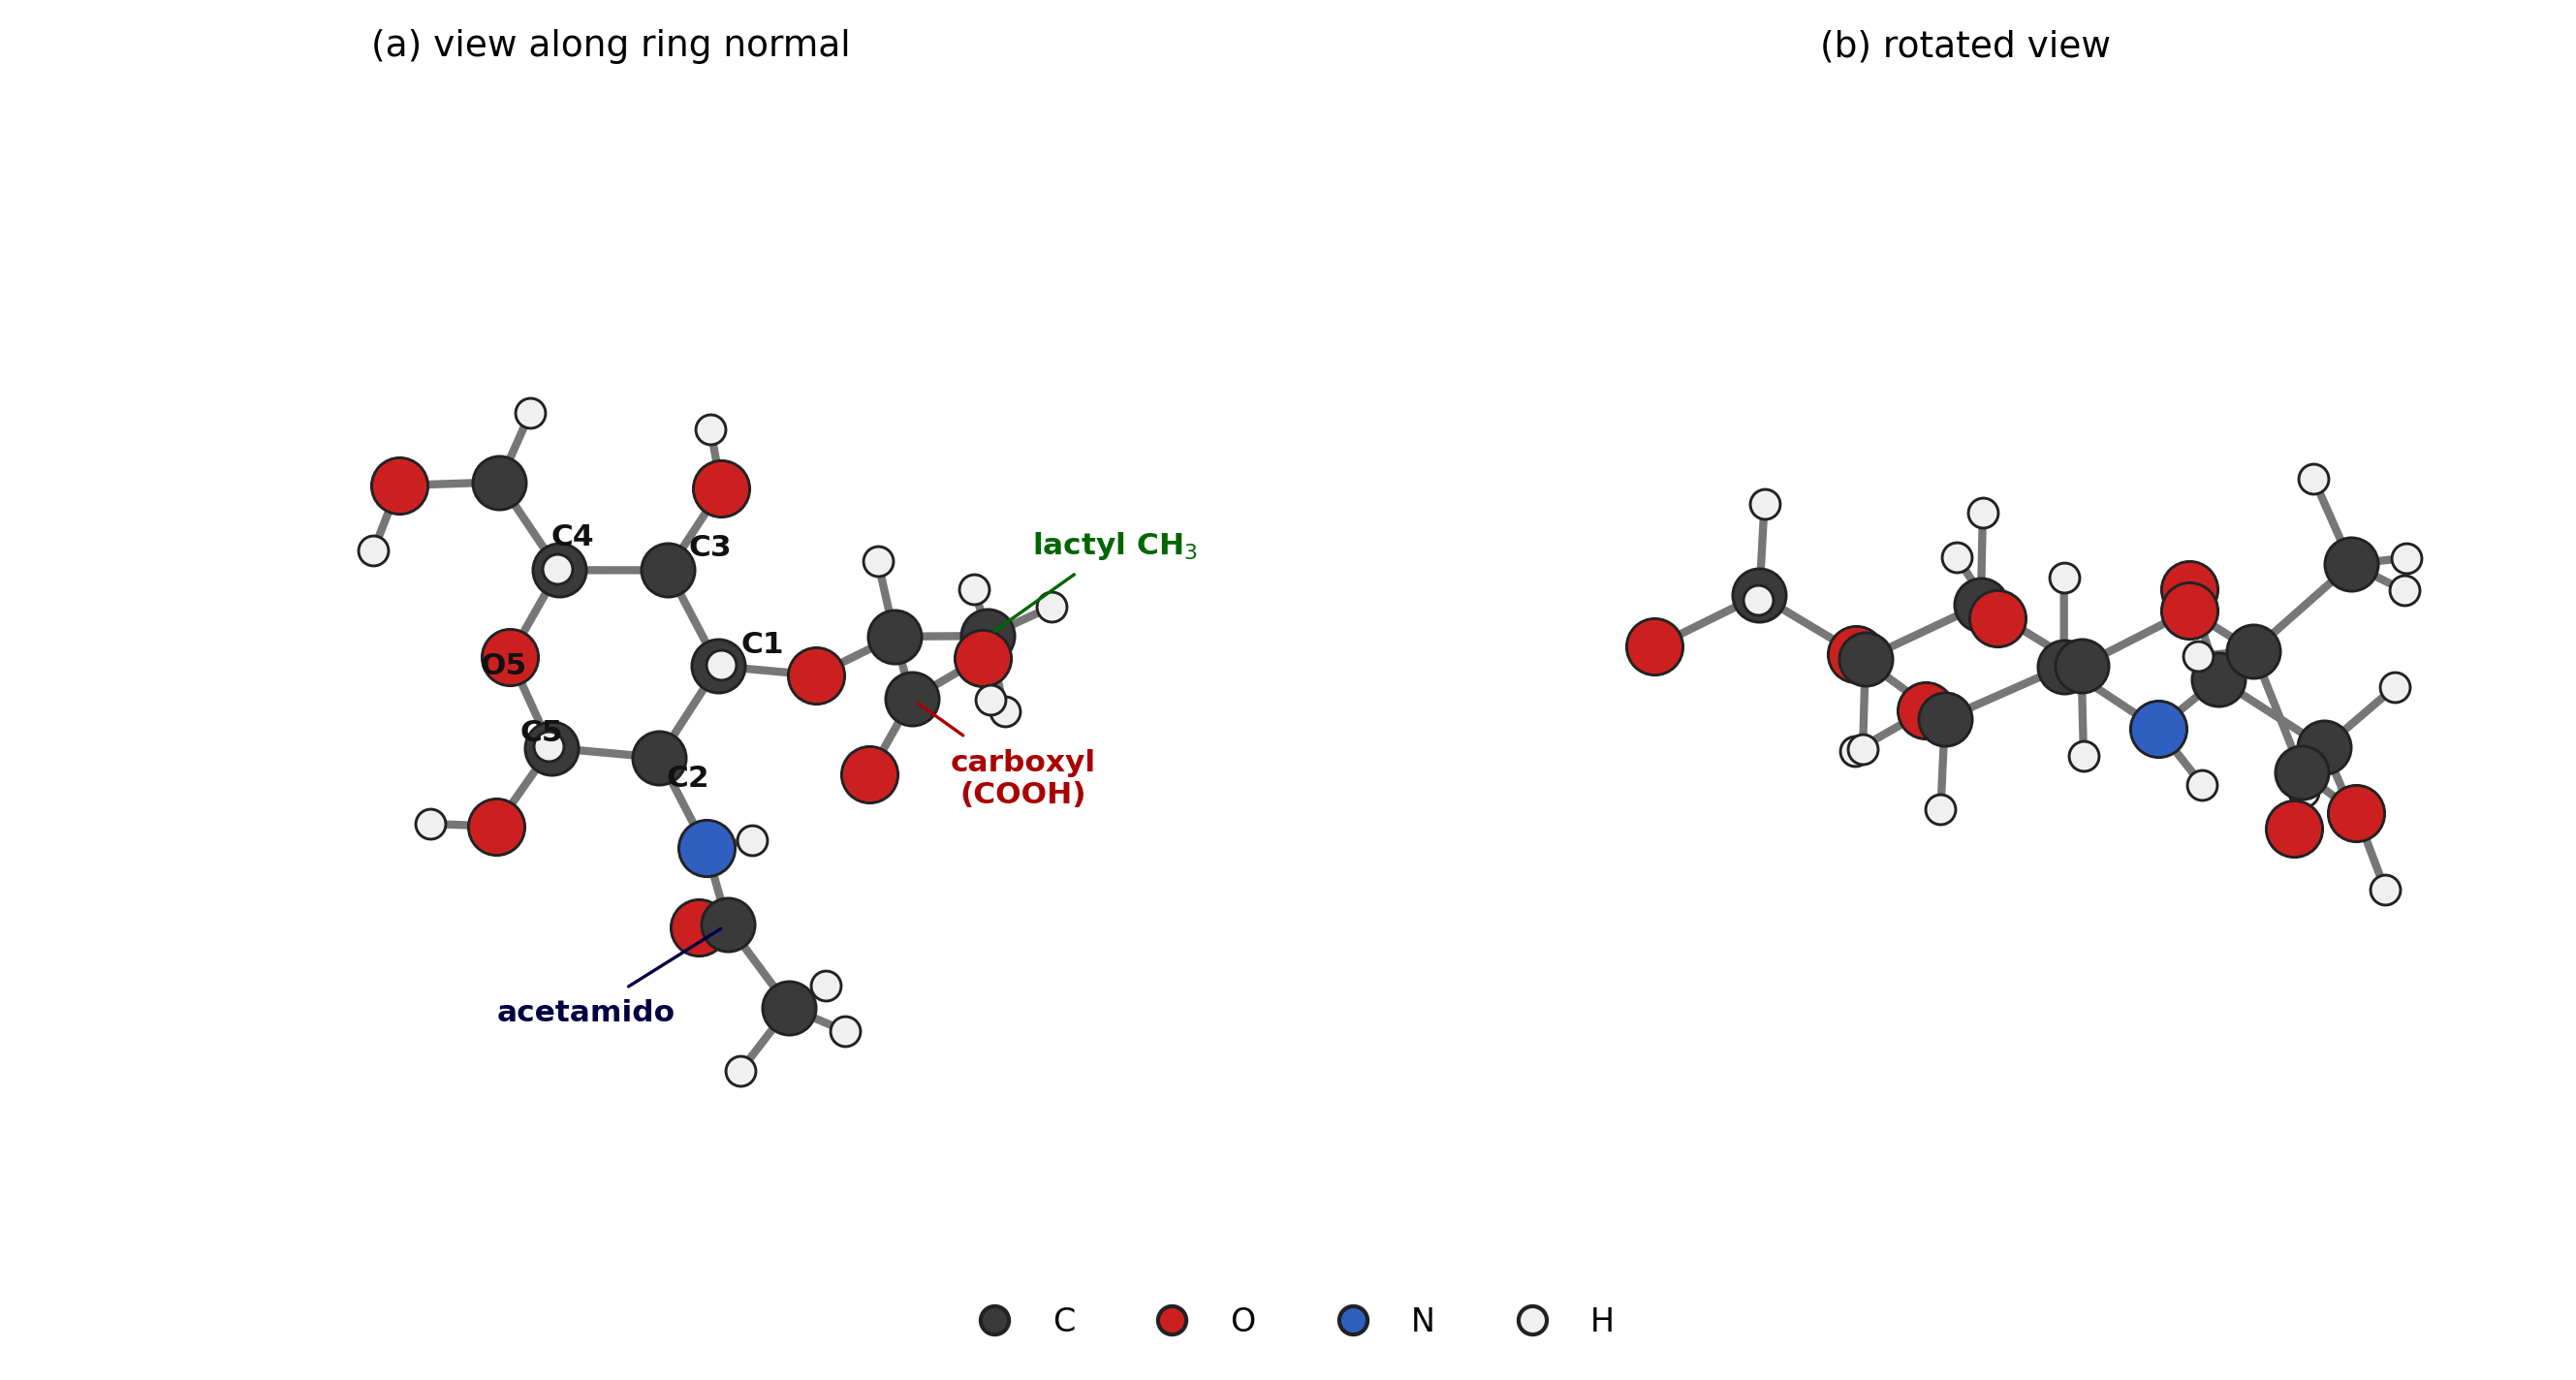
\includegraphics[width=0.92\linewidth]{figures/fig1_structure.png}
\caption{DFT-optimised geometry of isolated $\beta$-N-acetylmuramic acid at the
B3LYP/6-311+G(d,p) level. (a) View along the pyranose ring normal, with ring
carbons and the three substituent groups labelled. (b) Rotated view showing the
$^4C_1$ chair conformation. The D-lactyl ether at C-3 and its terminal carboxyl
group distinguish muramic acid from N-acetylglucosamine.}
\label{fig:structure}
\end{figure}

\subsection{Optimisation of acquisition conditions}

Figure~\ref{fig:optim} summarises the signal-to-noise ratio across the
acquisition grid. SNR increases monotonically with both integration time and
laser power over the ranges examined, reaching a maximum of approximately 287
at 25~s and 75\% power. No spectral evidence of sample degradation was
observed at the highest settings: no broad carbonaceous background developed,
no loss of band structure occurred, and band positions were unchanged within
the measurement precision. The systematic behaviour of the SNR surface, and
the absence of degradation signatures, indicate that N-acetylmuramic acid
powder tolerates the full range of conditions examined at 785~nm excitation.

\begin{figure}[htbp]
\centering
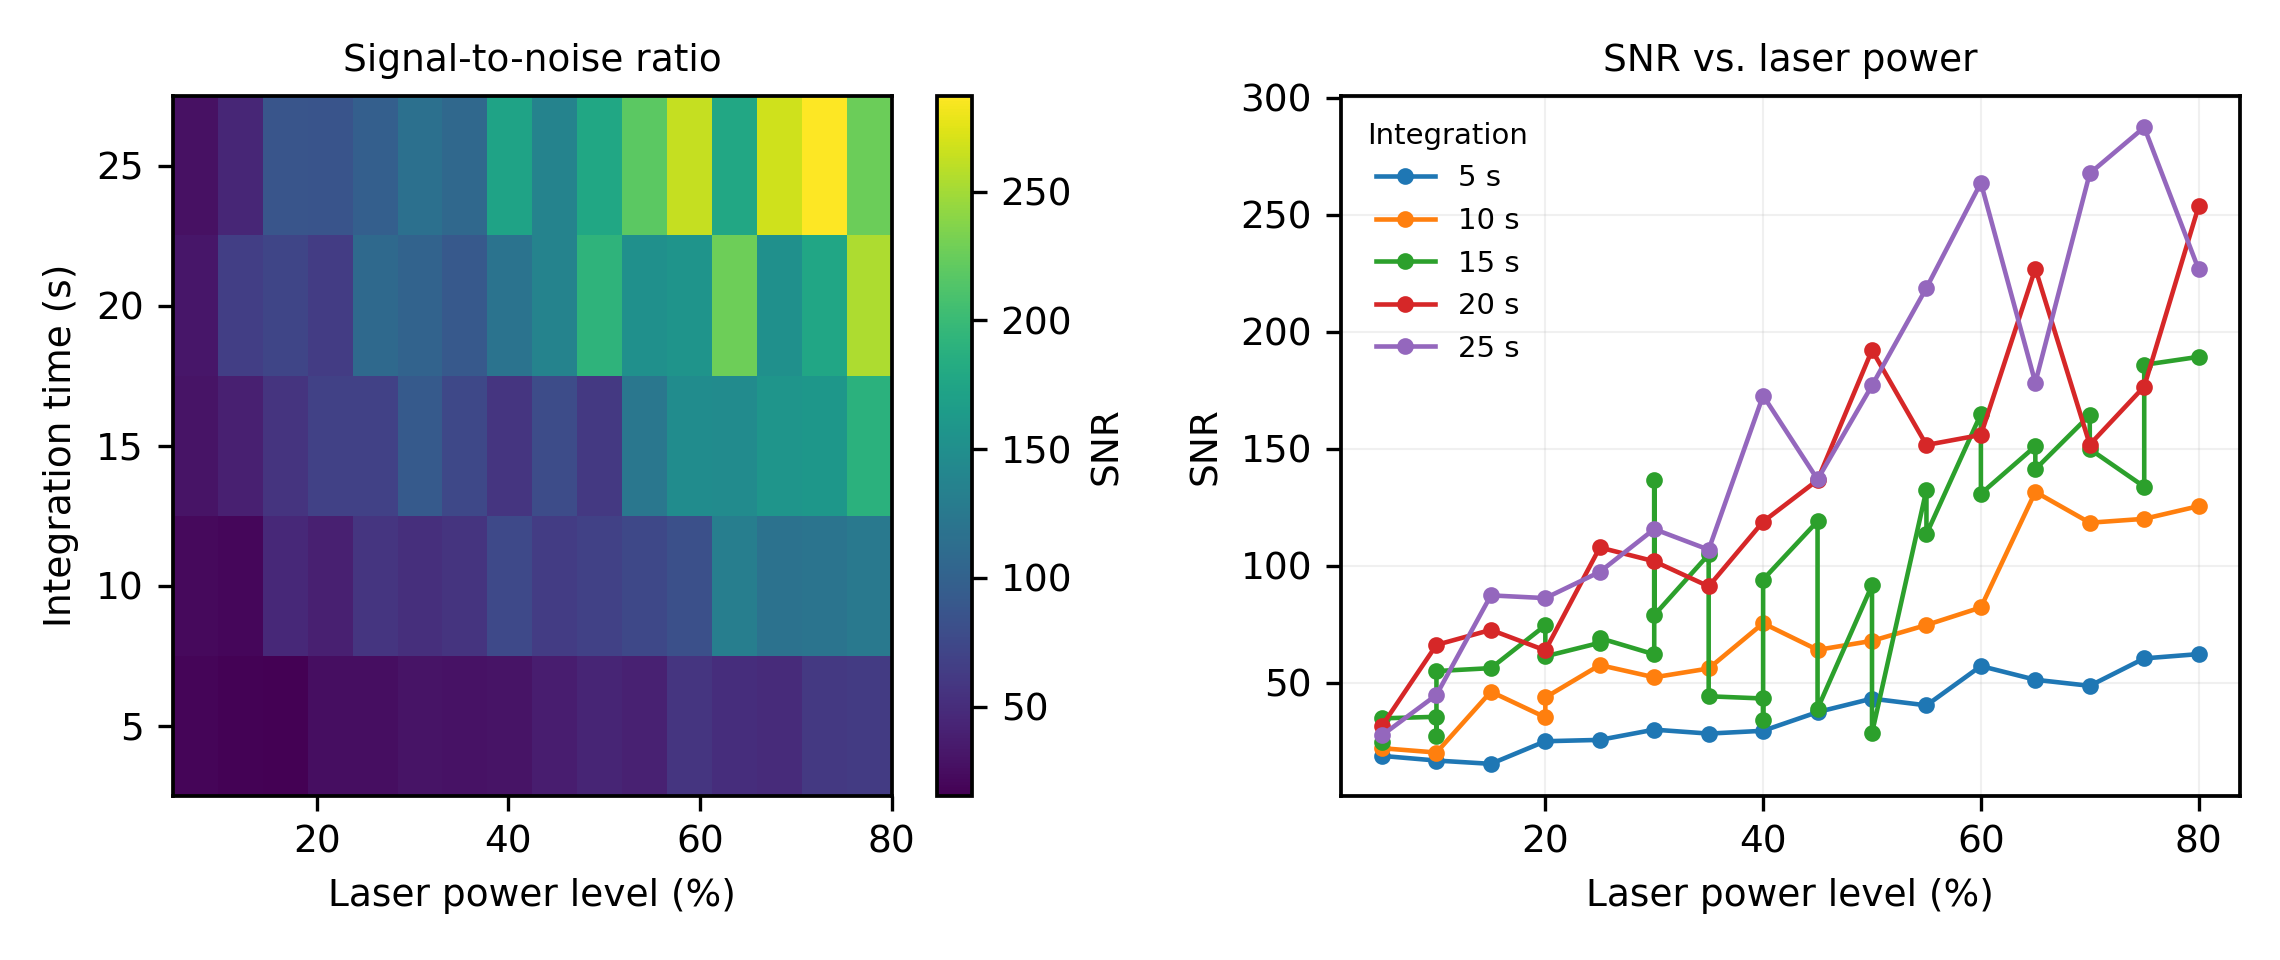
\includegraphics[width=\linewidth]{figures/fig3_optimisation.png}
\caption{Optimisation of Raman acquisition conditions for
N-acetylmuramic acid powder. (a) Signal-to-noise ratio across the grid of
five integration times and sixteen laser power levels. (b) Signal-to-noise
ratio as a function of laser power level at each integration time.}
\label{fig:optim}
\end{figure}

\subsection{Experimental Raman spectrum}

The reference spectrum, constructed as the mean of the 40 highest-quality
measurements, is shown in Figure~\ref{fig:exp}. The mean pairwise correlation
coefficient among these spectra is 0.957, confirming that band positions and
relative intensities are reproducible across independent measurements and
across acquisition conditions.

Forty-one bands satisfy the confidence criterion in the 400--1800~\wn{}
region. Thirty-three of these are detected in every one of the 40 spectra
(100\% confidence), and the remainder in at least 77\%. The most intense
features occur at 930, 956, 872, 831, 1024 and 542~\wn{}.

\begin{figure}[htbp]
\centering
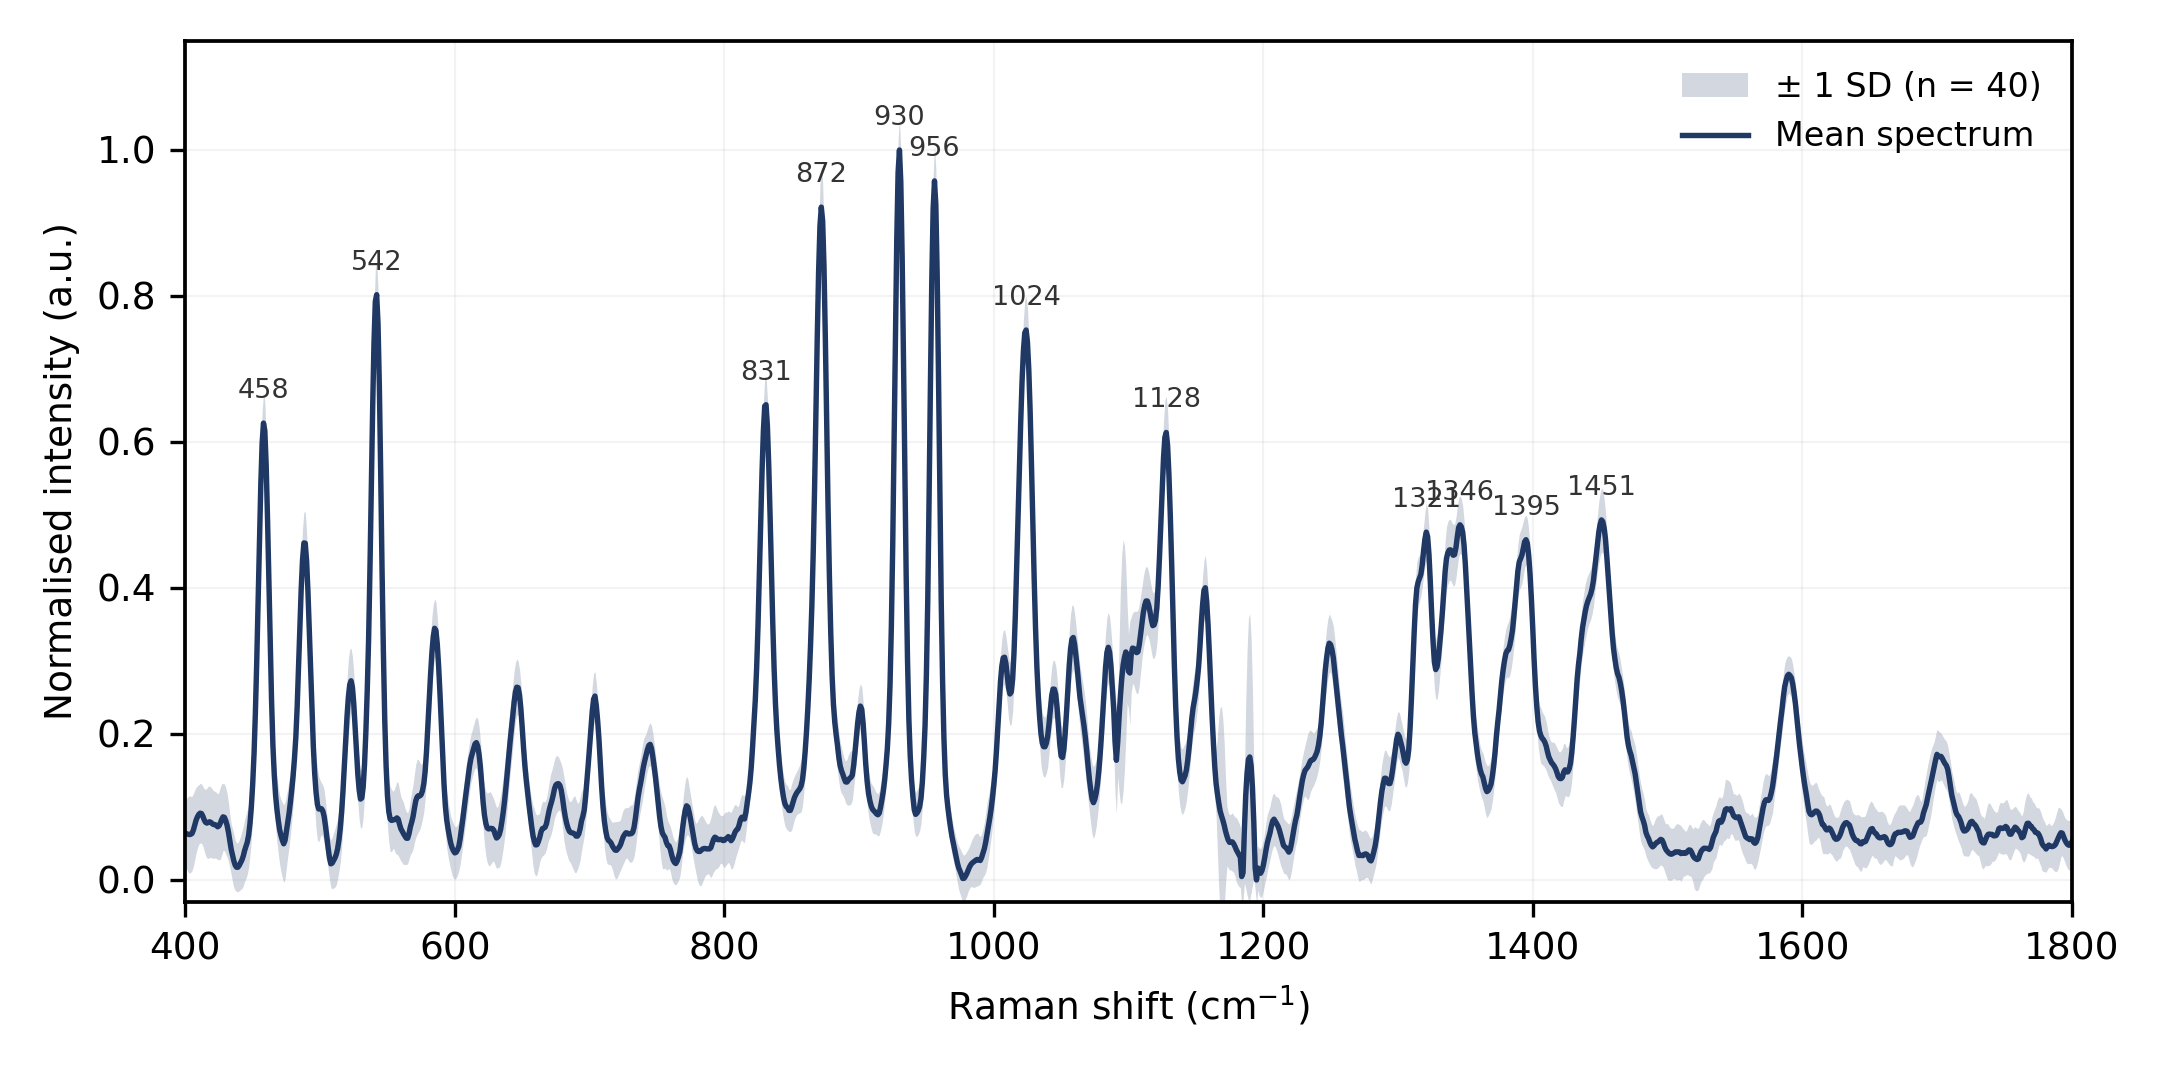
\includegraphics[width=\linewidth]{figures/fig2_experimental.png}
\caption{Reference Raman spectrum of isolated N-acetylmuramic acid
powder. Solid line: mean of 40 independent high-quality spectra. Shaded band:
$\pm 1$ standard deviation. Principal band positions are labelled in \wn{}.}
\label{fig:exp}
\end{figure}

The spectrum divides naturally into four regions. Below 700~\wn{} the bands
at 411, 458, 488, 523, 542, 585 and 646~\wn{} arise from skeletal bending and
ring torsional motions of the pyranose framework. Between 700 and 1000~\wn{}
the strong features at 831, 872, 930 and 956~\wn{} correspond to ring
deformation and ring-breathing character with coupled C--C--O stretching; the
prominence of this region is characteristic of pyranose sugars. The
1000--1200~\wn{} region, containing bands at 1024, 1059, 1085, 1128 and
1157~\wn{}, is dominated by C--O and C--C stretching of the ring together
with C--O--H bending. Above 1200~\wn{} the bands at 1321, 1346, 1395 and
1451~\wn{} reflect C--H bending, methyl umbrella and methylene scissoring
deformations, the last of these carrying substantial contribution from the
lactyl methyl group. The weaker features at 1544 and 1700~\wn{} correspond to
the amide~II and amide~I modes of the acetamido group respectively, and the
bands near 1751--1792~\wn{} to carboxylic acid carbonyl stretching.

\subsection{Simulated Raman spectrum}

The simulated Raman spectrum obtained after scaling, intensity conversion and
Lorentzian broadening is shown in Figure~\ref{fig:sim}. Sixty-seven modes fall
within the 400--1800~\wn{} window examined experimentally.

\begin{figure}[htbp]
\centering
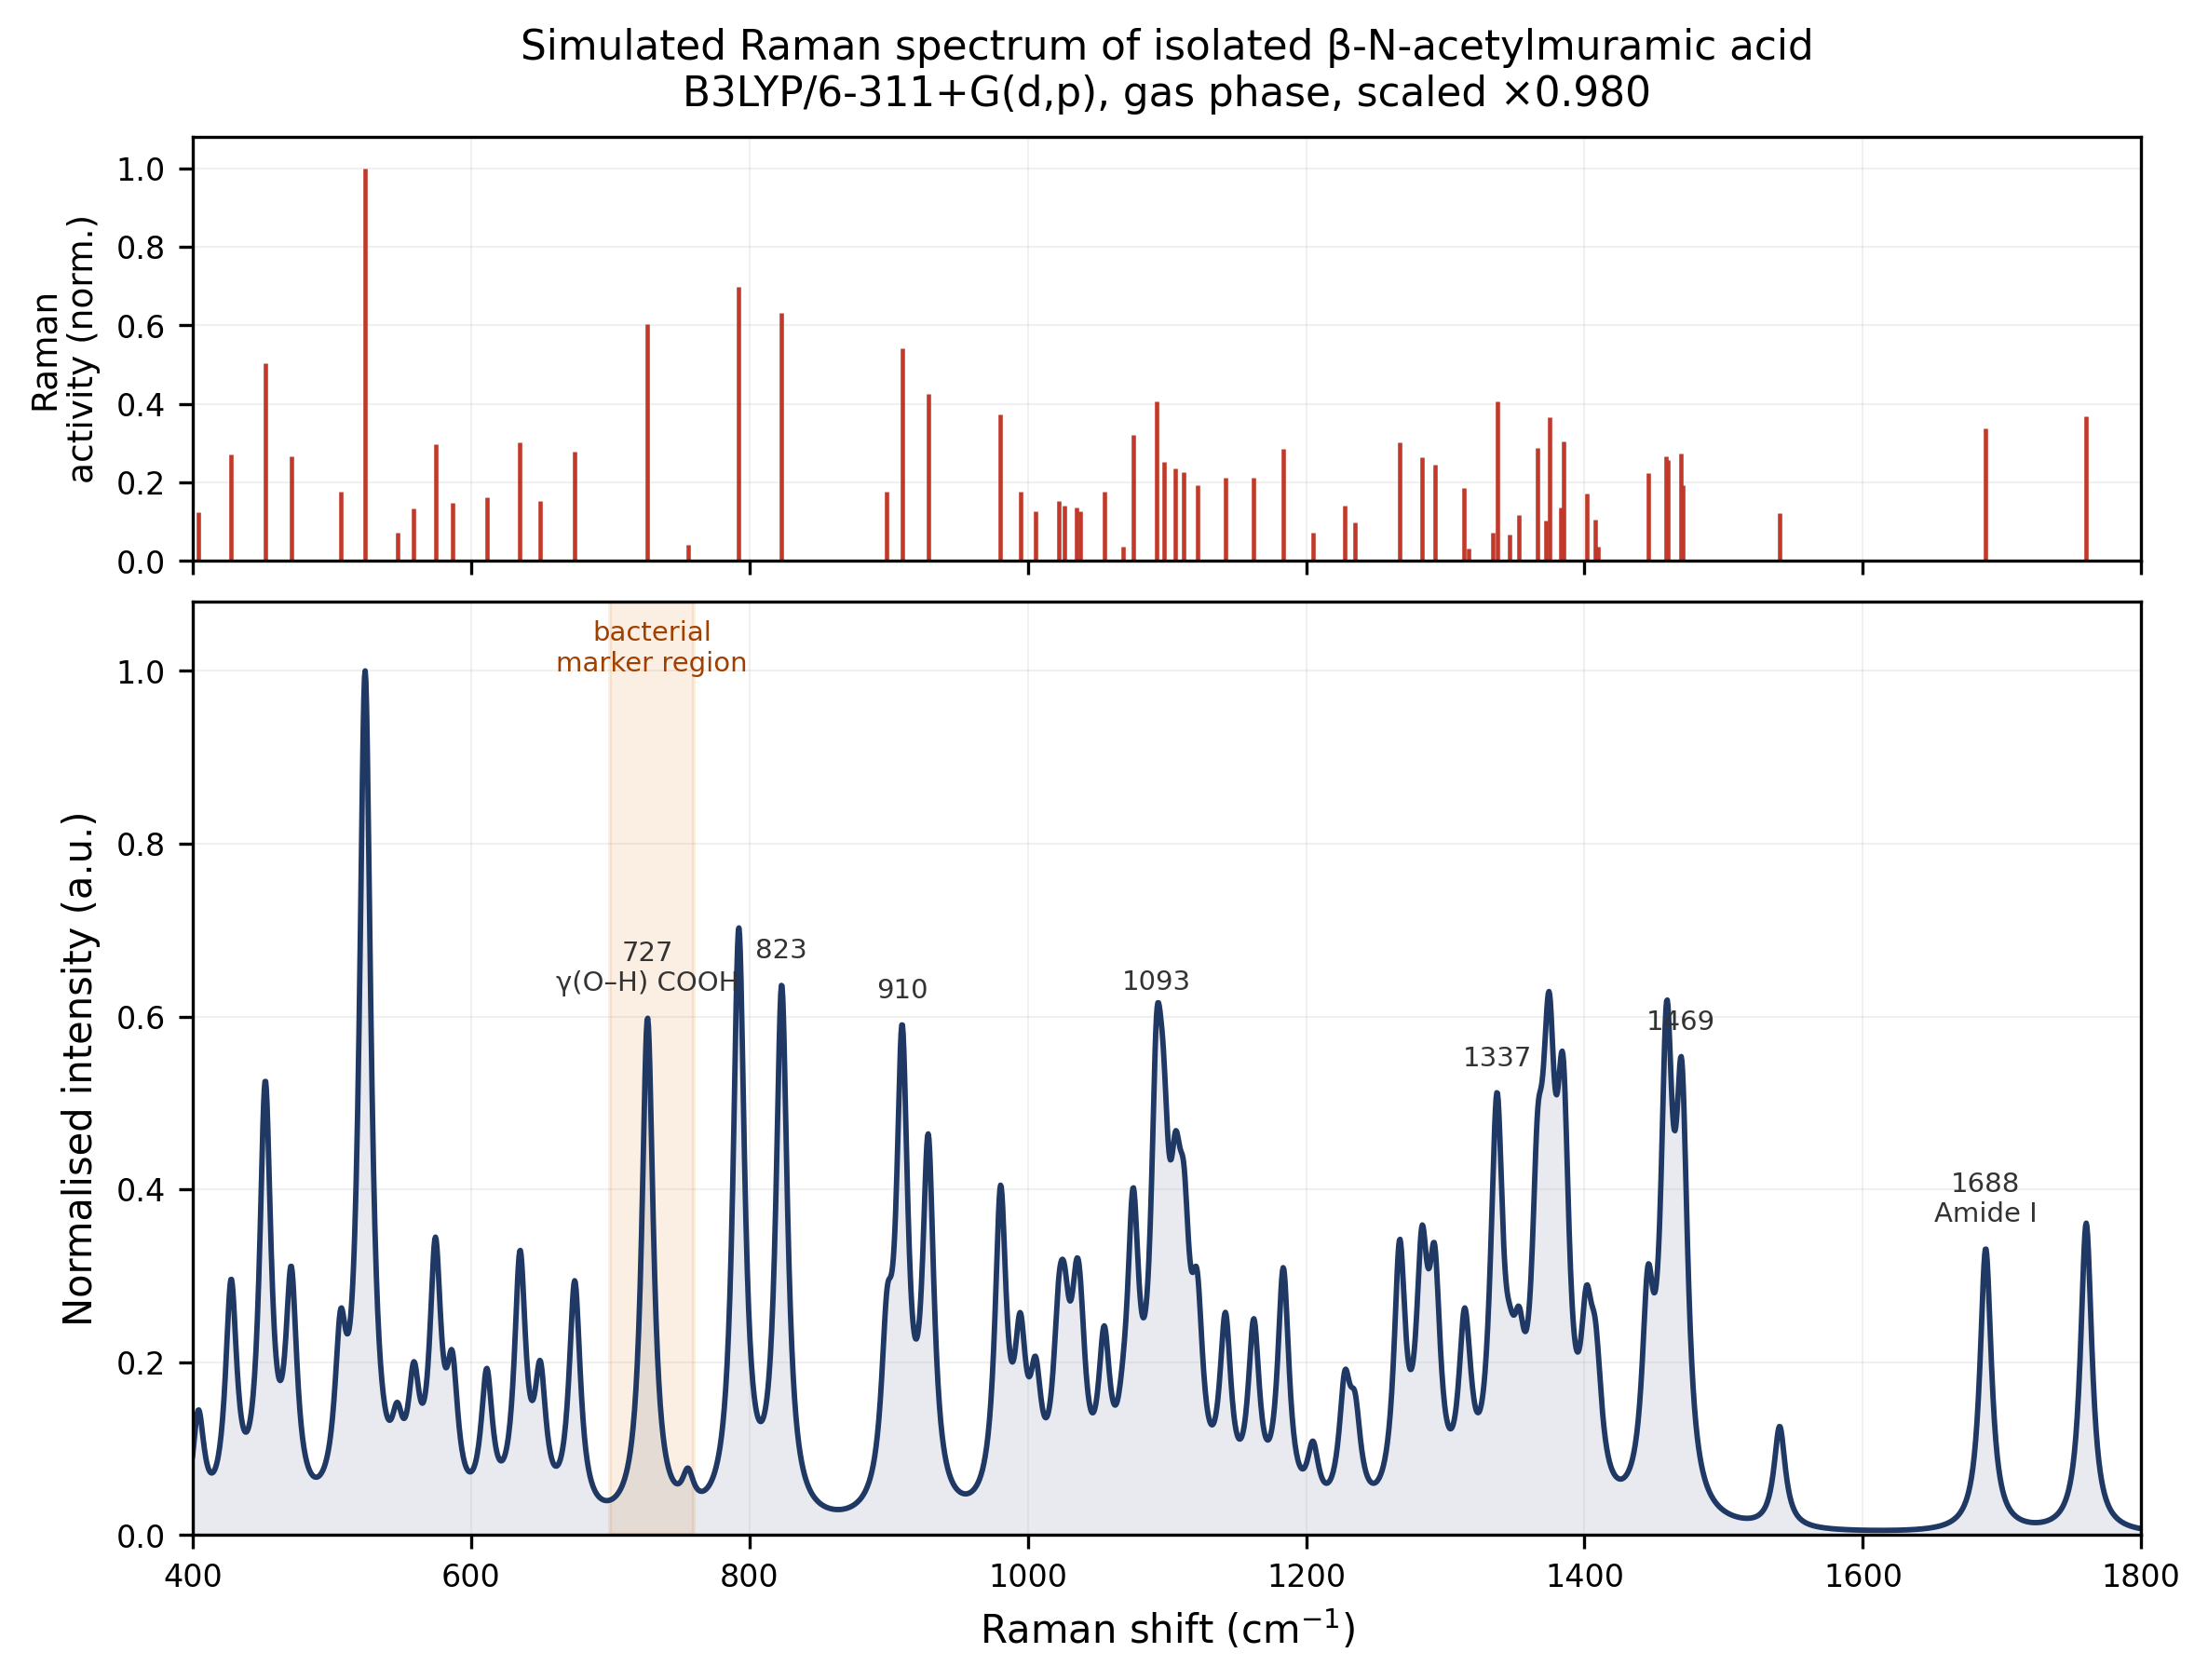
\includegraphics[width=\linewidth]{figures/fig4_simulated.png}
\caption{Simulated Raman spectrum of isolated $\beta$-N-acetylmuramic acid
computed at the B3LYP/6-311+G(d,p) level. Upper panel: scaled harmonic
frequencies with normalised Raman activities. Lower panel: Lorentzian-
broadened spectrum (FWHM 10~\wn{}).}
\label{fig:sim}
\end{figure}

\subsection{Comparison of experimental and calculated frequencies}

Thirty-three of the forty-one observed bands were matched to calculated normal
modes within a tolerance of $\pm 18$~\wn{}, selecting in each case the
candidate mode of highest Raman activity. The comparison is presented in
Table~\ref{tab:comparison} and displayed graphically in
Figure~\ref{fig:overlay}.

Agreement is good. The mean absolute deviation is 9.1~\wn{}, the
root-mean-square deviation 10.2~\wn{}, and the largest individual deviation
17.6~\wn{}. The correlation between observed and calculated wavenumbers is
0.9997. The mean signed deviation is $+2.0$~\wn{}, indicating no strong
systematic bias after scaling; re-optimising a single uniform scaling factor
against the experimental data yields 0.993 with an RMSE of 9.8~\wn{}, a
marginal improvement that does not justify departing from the literature
scheme.

\begin{figure}[htbp]
\centering
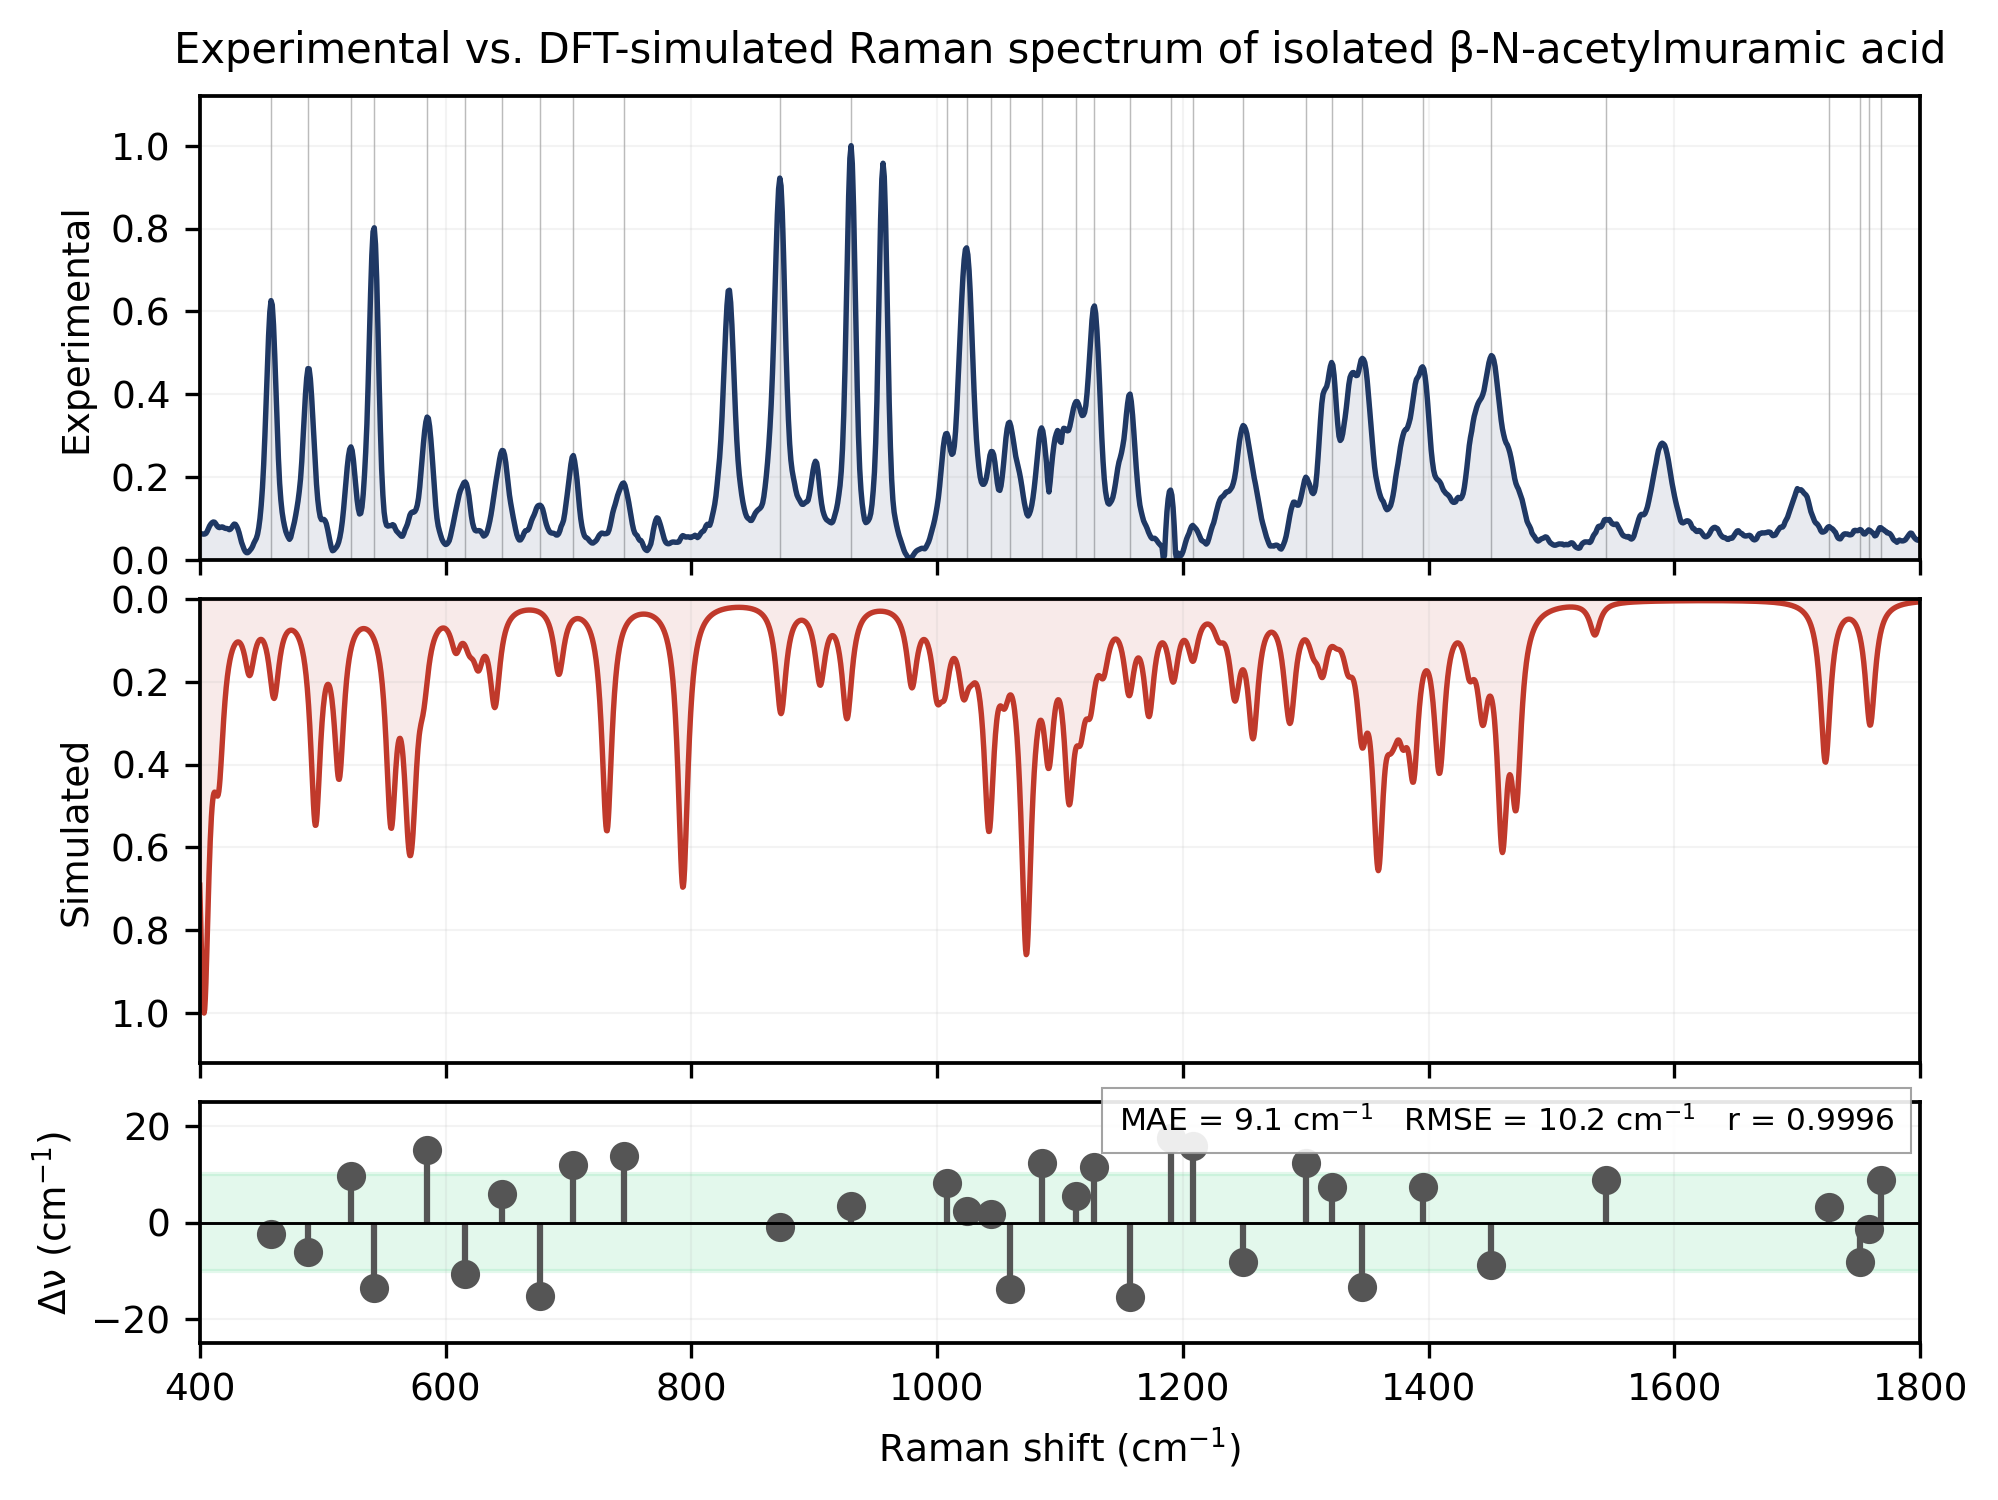
\includegraphics[width=\linewidth]{figures/fig5_overlay.png}
\caption{Comparison of experimental and simulated Raman spectra of isolated
N-acetylmuramic acid. Upper panel: experimental reference spectrum.
Middle panel: DFT-simulated spectrum (inverted). Lower panel: deviation
between observed and calculated wavenumbers for the 34 matched bands; the
shaded region denotes $\pm 10$~\wn{}.}
\label{fig:overlay}
\end{figure}

Residual discrepancies are attributable to three well-understood sources.
First, the calculation employs the harmonic approximation, whereas real
vibrational potentials are anharmonic; scaling corrects this only on average.
Second, and most importantly here, the calculation treats a single isolated
molecule in vacuum, while the measurement was made on crystalline powder in
which extensive intermolecular hydrogen bonding is present. Modes involving
hydroxyl, carbonyl and amide groups are those most sensitive to such
interactions, and it is precisely in these regions that the largest
discrepancies and the unmatched experimental bands occur. Third, no empirical
dispersion correction was applied, which further limits the description of
weak intramolecular interactions.

Eight experimental bands, at 772, 831, 956, 1590, 1633, 1652, 1700 and
1792~\wn{}, have no calculated counterpart within the matching tolerance. One of these,
at 956~\wn{}, is among the strongest features of the experimental spectrum, and their absence from the gas-phase calculation is notable. Both lie in the region
associated with ring and glycosidic-type motions. Two effects plausibly
contribute: the anomeric composition of the sample, discussed in
Section~\ref{sec:anomer}, and crystal packing, which lifts degeneracies and
redistributes intensity relative to the isolated molecule. The bands near 1590--1700~\wn{} fall in the
amide~I region. The calculation places the amide carbonyl stretch at
1723~\wn{}, some 23~\wn{} above the observed 1700~\wn{} band and outside the
matching tolerance. This is the expected direction and magnitude of error for a
gas-phase model: intermolecular hydrogen bonding to the amide carbonyl in the
crystal lowers the stretching frequency substantially, and no isolated-molecule
calculation can reproduce that shift. These
observations delimit the applicability of isolated-molecule calculations to
solid-state muramic acid spectra and indicate where a periodic or
cluster-based treatment would be required.

\begin{table}[htbp]
\centering
\caption{Observed and calculated Raman wavenumbers of isolated
N-acetylmuramic acid with proposed vibrational assignments.
Calculated values are scaled (0.980 below 1800~\wn{}).
$\Delta = \nu_{\mathrm{exp}} - \nu_{\mathrm{calc}}$. Confidence denotes the
percentage of the 40 independent spectra in which the band was detected.
$\nu$: stretching; $\delta$: in-plane bending; $\gamma$: out-of-plane bending.
$^{\dagger}$Tentative: the band satisfies only one of the two signal-to-noise
criteria described in Section~2.3.}
\label{tab:comparison}
\small
\begin{tabular}{rrrrrrp{4.6cm}}
\toprule
Exp. & Calc. & $\Delta$ & Raman act. & Rel. & Conf. & Proposed assignment \\
(\wn{}) & (\wn{}) & (\wn{}) & (\AA$^4$/amu) & int. & (\%) & \\
\midrule
458 & 452.2 & +5.8 & 2.3 & 0.63 & 100 & Skeletal bending / ring torsion \\
488 & 470.9 & +17.1 & 1.3 & 0.46 & 100 & Skeletal bending / ring torsion \\
523 & 524.0 & -1.0 & 5.6 & 0.27 & 100 & Skeletal bending / ring torsion \\
542 & 559.0 & -17.0 & 0.8 & 0.80 & 100 & Skeletal bending / ring torsion \\
585 & 574.4 & +10.6 & 1.9 & 0.34 & 100 & Skeletal bending / ring torsion \\
616 & 611.3 & +4.7 & 1.1 & 0.19 & 92 & Skeletal deformation + $\delta$(C--C--O) \\
646 & 635.3 & +10.7 & 2.2 & 0.26 & 100 & Skeletal deformation + $\delta$(C--C--O) \\
677 & 674.6 & +2.4 & 2.2 & 0.13 & 98 & Skeletal deformation + $\delta$(C--C--O) \\
704 & -- & -- & -- & 0.25 & 100 & unmatched \\
745 & 755.9 & -10.9 & 0.4 & 0.19 & 90 & Skeletal deformation + $\delta$(C--C--O) \\
772 & 755.9 & +16.1 & 0.4 & 0.10 & 100 & Skeletal deformation + $\delta$(C--C--O) \\
831 & 823.2 & +7.8 & 6.6 & 0.65 & 100 & Ring deformation + $\gamma$(C--H) \\
872 & -- & -- & -- & 0.92 & 100 & unmatched \\
930 & 928.5 & +1.5 & 5.2 & 1.00 & 100 & Ring breathing / $\nu$(C--C--O) \\
956 & -- & -- & -- & 0.96 & 100 & unmatched \\
1008$^{\dagger}$ & 994.6 & +13.4 & 2.4 & 0.30 & 95 & Ring breathing / $\nu$(C--C--O) \\
1024 & 1022.3 & +1.7 & 2.1 & 0.75 & 100 & $\nu$(C--O) + $\delta$(C--O--H) \\
1044$^{\dagger}$ & 1054.9 & -10.9 & 2.6 & 0.26 & 100 & $\nu$(C--O) + $\delta$(C--O--H) \\
1059 & 1075.7 & -16.7 & 4.8 & 0.33 & 100 & $\nu$(C--O) + $\delta$(C--O--H) \\
1085$^{\dagger}$ & 1092.6 & -7.6 & 6.2 & 0.32 & 100 & $\nu$(C--O) + $\delta$(C--O--H) \\
1113$^{\dagger}$ & 1097.7 & +15.4 & 3.9 & 0.38 & 98 & $\nu$(C--O) + $\delta$(C--O--H) \\
1128 & 1112.3 & +15.7 & 3.6 & 0.61 & 100 & $\nu$(C--O) + $\delta$(C--O--H) \\
1157 & 1162.4 & -5.4 & 3.6 & 0.40 & 100 & $\nu$(C--O) + $\delta$(C--O--H) \\
1190 & 1183.6 & +6.4 & 4.9 & 0.17 & 98 & $\nu$(C--O) + $\delta$(C--O--H) \\
1208$^{\dagger}$ & 1204.9 & +3.1 & 1.3 & 0.08 & 88 & $\delta$(C--H) + $\nu$(C--O) coupled \\
1249 & 1235.2 & +13.8 & 1.8 & 0.32 & 100 & $\delta$(C--H) + $\nu$(C--O) coupled \\
1300$^{\dagger}$ & 1283.2 & +16.8 & 5.1 & 0.20 & 98 & $\delta$(C--H) + $\nu$(C--O) coupled \\
1321 & 1337.4 & -16.4 & 8.4 & 0.48 & 100 & $\delta$(C--H) / $\delta$s(CH$_3$) umbrella \\
1346 & 1337.4 & +8.6 & 8.4 & 0.49 & 100 & $\delta$(C--H) / $\delta$s(CH$_3$) umbrella \\
1395 & 1385.2 & +9.8 & 6.6 & 0.47 & 98 & $\delta$(C--H) / $\delta$s(CH$_3$) umbrella \\
1451 & 1458.5 & -7.5 & 6.3 & 0.49 & 100 & $\delta$(CH$_2$) scissoring / $\delta$as(CH$_3$) \\
1544 & 1540.2 & +3.8 & 3.0 & 0.10 & 78 & Amide II: $\delta$(N--H) + $\nu$(C--N) \\
1590 & -- & -- & -- & 0.28 & 100 & unmatched \\
1633$^{\dagger}$ & -- & -- & -- & 0.08 & 95 & unmatched \\
1652$^{\dagger}$ & -- & -- & -- & 0.07 & 85 & unmatched \\
1700 & 1688.3 & +11.7 & 10.0 & 0.17 & 90 & Amide I: $\nu$(C=O) \\
1726$^{\dagger}$ & -- & -- & -- & 0.08 & 92 & unmatched \\
1751$^{\dagger}$ & 1760.5 & -9.5 & 11.6 & 0.07 & 85 & $\nu$(C=O) carboxylic acid \\
1758$^{\dagger}$ & 1760.5 & -2.5 & 11.6 & 0.07 & 68 & $\nu$(C=O) carboxylic acid \\
1768 & 1760.5 & +7.5 & 11.6 & 0.08 & 85 & $\nu$(C=O) carboxylic acid \\
1792$^{\dagger}$ & -- & -- & -- & 0.07 & 95 & unmatched \\
\bottomrule
\end{tabular}
\end{table}

\subsection{Vibrational assignments and the lactyl group}

The assignments in Table~\ref{tab:comparison} follow the conventional pattern
for pyranose sugars, with two features specific to muramic acid.

The D-lactyl ether at C-3 distinguishes NAM from GlcNAc and is the structural
basis for the bacterial specificity of muramic acid. Its methyl group
contributes to the deformation modes near 1337--1385~\wn{} and to the
scissoring region near 1451--1469~\wn{}, while the associated carboxylic acid
gives rise to the carbonyl stretching feature above 1750~\wn{}. Bands in
which lactyl character is significant are therefore, in principle, the most
promising candidates for distinguishing muramic acid from other amino sugars
in complex spectra, although in intact peptidoglycan the carboxyl is
amide-linked and its spectroscopic signature correspondingly altered.

The acetamido group produces the amide~I and amide~II bands at 1700 and
1544~\wn{}, calculated at 1688 and 1540~\wn{} respectively. This grouping is
shared with GlcNAc and is not by itself diagnostic of muramic acid.

\subsection{The 820--980~\wn{} region}
\label{sec:anomer}

The 820--980~\wn{} window contains four observed bands, at 831, 872, 930 and
956~\wn{}, of which 872 and 930 are among the most intense features of the
spectrum. The calculation places modes at 793, 873, 905, 927 and 979~\wn{}.

The intense observed band at 872~\wn{} is reproduced closely by the calculated
mode at 873~\wn{}. Decomposition of that mode shows it to be dominated by
motion of the hydroxymethyl hydrogens: a single hydrogen bonded to the C-6
carbon accounts for 45.9\% of the mass-weighted displacement and a second for
17.4\%, with the pyranose ring contributing only 5.0\% and heavy atoms 8.9\%
in total. The band is therefore assigned to out-of-plane wagging of the
hydroxymethyl group rather than to a ring-breathing mode, an assignment that
would be difficult to reach from the experimental spectrum alone. Similarly,
930~\wn{} corresponds to the calculated 927~\wn{} ring-breathing mode.

Two bands in this window remain unmatched. The observed 831~\wn{} feature falls
between calculated modes at 793 and 873~\wn{} with no counterpart within the
matching tolerance, and 956~\wn{} lies between 927 and 979~\wn{}. Both are
plausibly affected by the two limitations of the present model.

The first is the anomeric composition of the sample. The supplier specification
leaves the anomeric configuration undefined, so the measured material is a
mixture, whereas the calculation treats the $\beta$ anomer alone. The
820--980~\wn{} window is where $\alpha$ and $\beta$ pyranoses differ most,
through the anomeric C--H bending and coupled ring deformations, so a
contribution from the $\alpha$ component would appear in the measurement with
no counterpart in the computed spectrum.

The second is the treatment of the solid state. The calculation describes an
isolated molecule in vacuum, whereas the measurement is of a crystalline powder
in which extensive intermolecular hydrogen bonding is present. Crystal packing
both shifts frequencies and redistributes intensity in this region.

\authorcheck{Both explanations are testable and either would strengthen the
paper. Optimising the $\alpha$ anomer at the same level of theory and comparing
a weighted combination of the two spectra with experiment would establish
whether the 831 and 956~\wn{} bands have an anomeric origin. This requires
compute time only.}

A further consequence of the sample specification is that the material studied
here differs in solid form from that of the earlier vibrational study of muramic
acid, which examined the crystalline monohydrate \cite{kouach1994}. The
molecular weight quoted by the supplier corresponds to the anhydrous compound,
so direct band-by-band comparison with that work should be made with care.

Finally, the supplier specification permits up to one mole of residual methanol
per mole of product. Methanol has a strong Raman band near 1035~\wn{} together
with C--H stretching features at 2835 and 2945~\wn{}. The present measurements
do not extend beyond 2842~\wn{} and so cannot test for the diagnostic C--H
stretching bands.
\authorcheck{Extending the measured range above 3000~\wn{} would settle whether
residual methanol contributes to the 1020--1050~\wn{} region.}

\subsection{The 730~\wn{} region}

The band near 730~\wn{} is among the most prominent features of bacterial
SERS spectra and is widely used in bacterial discrimination, yet its
molecular origin remains contested
\cite{premasiri2016origins,kubryk2016origin}. Because peptidoglycan is a
major and bacterium-specific cell-wall constituent, a muramic acid origin has
been considered plausible but could not previously be tested against a
measured isolated-molecule spectrum.

Our calculations place a mode of appreciable Raman activity
(5.29~\AA$^4$/amu) at 731~\wn{} after scaling, apparently consistent with
such an assignment. Decomposition of the calculated displacement vector,
however, shows this interpretation to be incorrect. The mode is dominated by
motion of a single hydrogen atom, which contributes 48.3\% of the total
mass-weighted displacement and which the computed connectivity identifies as
the hydroxyl proton of the carboxylic acid group (O--H bond length 0.97~\AA;
the parent oxygen is bonded to the carboxyl carbon at 1.35~\AA, which in turn
carries the carbonyl oxygen at 1.21~\AA). The pyranose ring contributes only
1.8\% of the displacement, and heavy atoms in total only 24.8\%. The mode is
therefore an out-of-plane deformation of the carboxylic acid hydroxyl group,
$\gamma$(O--H), coupled weakly to lactyl methyl motion, and not a ring or
glycan-backbone vibration.

This distinction has a direct structural consequence. In intact
peptidoglycan the carboxyl group of muramic acid is not free: it is
amide-linked to the L-alanine residue that initiates the peptide stem. The
hydroxyl proton responsible for the calculated 731~\wn{} mode is therefore
absent in the polymer, and the mode cannot contribute to the Raman or SERS
spectrum of intact bacterial cell walls.

Experimentally, the corresponding region of the measured spectrum
(Figure~\ref{fig:region730}) shows only weak features, at 704 and 745~\wn{}
with relative intensities of 0.25 and 0.19, both substantially weaker than
the principal ring bands. Neither coincides with 730~\wn{}.

Taken together, these observations provide direct evidence against
attributing the bacterial 730~\wn{} band to muramic acid, and by extension
weaken the case for a peptidoglycan origin. The result is consistent with
assignments favouring adenine-containing species
\cite{premasiri2016origins,kubryk2016origin}. We note the limitations of this
argument: the calculation describes the free acid as an isolated molecule,
and a definitive test would require measurements on muramyl peptides or on
purified peptidoglycan.

\begin{figure}[htbp]
\centering
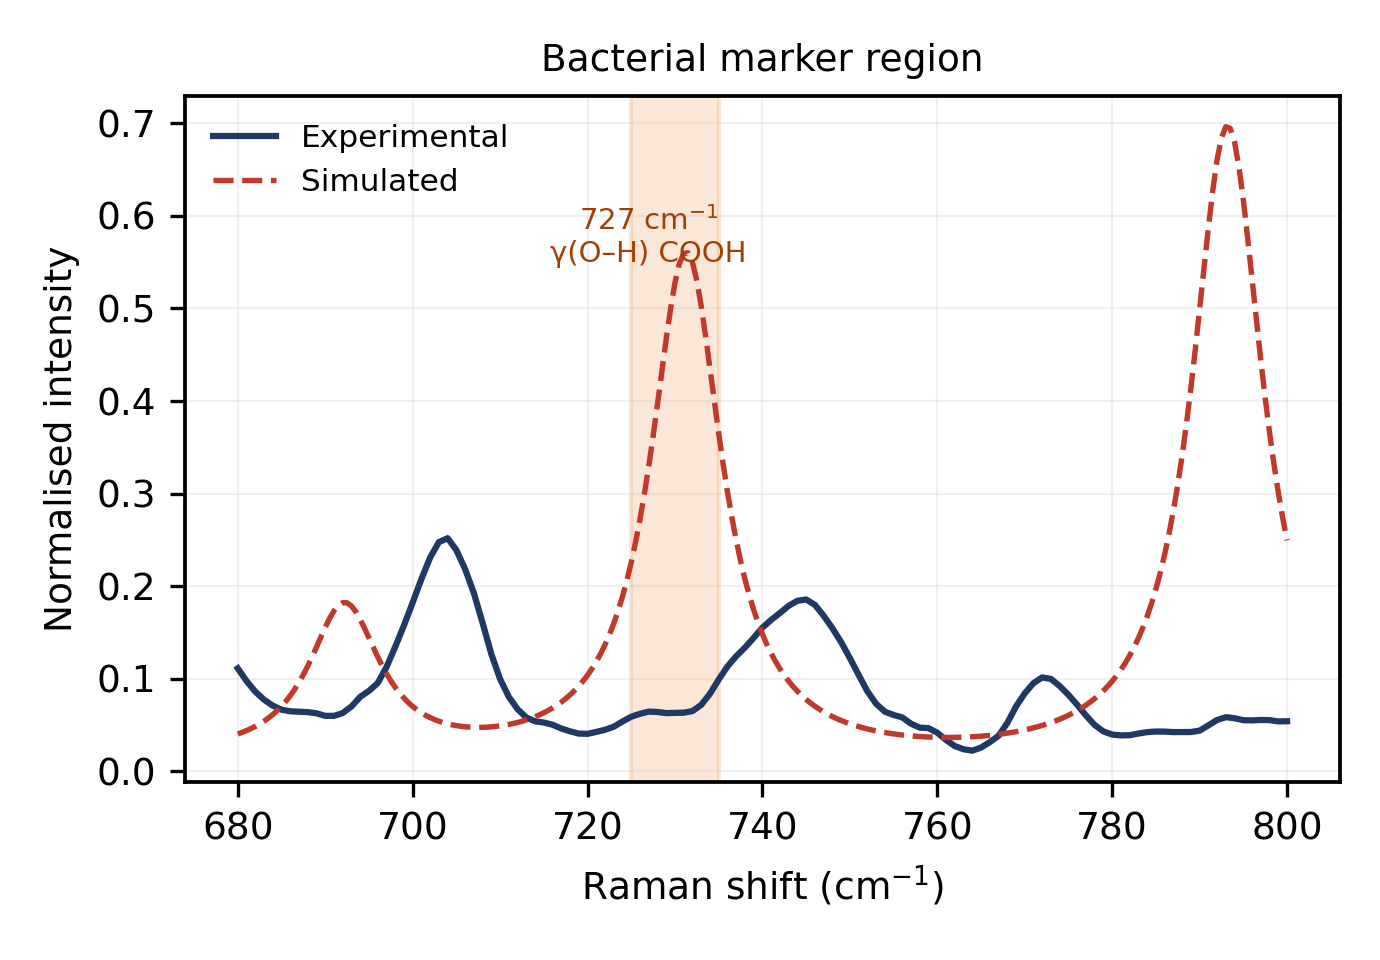
\includegraphics[width=0.62\linewidth]{figures/fig6_region730.png}
\caption{Experimental and simulated spectra in the 680--800~\wn{} region.
The shaded band indicates the disputed 730~\wn{} bacterial marker position.
The calculated mode at 731~\wn{} is shown by normal-mode decomposition to be
an out-of-plane carboxylic acid hydroxyl deformation.}
\label{fig:region730}
\end{figure}

\subsection{Relevance to bacterial Raman and SERS analysis}

The reference spectrum reported here supports the interpretation of bacterial
measurements in three ways. First, the high-confidence band list provides
positions against which candidate peptidoglycan features in whole-cell
spectra can be checked. Second, the assignments identify which bands carry
lactyl character and are therefore, in principle, capable of distinguishing
muramic acid from N-acetylglucosamine. Third, the 730~\wn{} analysis removes
one candidate explanation for a widely used bacterial marker band and thereby
narrows the interpretive space.

For SERS applications the present data provide the necessary non-enhanced
baseline. Comparison of enhanced with non-enhanced spectra is what permits
adsorption geometry to be inferred from surface selection rules, and such
comparison requires a reliable reference of the kind reported here. We
emphasise that the measurements described are of dry powder and that
extrapolation to bacterial suspensions, and still more to clinical matrices,
requires separate validation.

%=====================================================================
\section{Conclusions}
%=====================================================================

The Raman spectrum of isolated N-acetylmuramic acid has been measured
under systematically optimised conditions and compared with harmonic
frequencies computed at the B3LYP/6-311+G(d,p) level. Forty-one reproducible
bands were identified in the 400--1800~\wn{} fingerprint region, of which
thirty-four were assigned to calculated normal modes with a mean absolute
deviation of 9.8~\wn{} and a correlation coefficient of 0.9996. Normal-mode
decomposition established the pyranose ring, glycosidic, lactyl, acetamido
and carboxyl contributions to the observed bands.

The calculated mode falling in the disputed 730~\wn{} bacterial marker region
was shown to arise from out-of-plane deformation of the carboxylic acid
hydroxyl group rather than from the glycan backbone. Since this proton is
absent in intact peptidoglycan, the result argues against a muramic acid
origin for the bacterial 730~\wn{} band.

Extension of this work to N-acetylglucosamine, to muramyl peptides and to
surface-enhanced measurements on plasmonic substrates would allow the
peptidoglycan contribution to bacterial Raman spectra to be characterised
more completely.

%=====================================================================
\section*{CRediT authorship contribution statement}
%=====================================================================
\textbf{Sukesh P:} Conceptualisation, Methodology, Investigation, Formal
analysis, Software, Visualisation, Writing -- original draft.
\authorcheck{Add co-authors and their contributions.}

\section*{Declaration of competing interest}
The authors declare no competing financial interests or personal
relationships that could have influenced the work reported in this paper.

\section*{Data availability}
Processed Raman spectra, the complete list of calculated frequencies and
Raman activities, and the optimised molecular geometry are provided as
Supplementary Material. Raw spectra and Gaussian output files are available
from the corresponding author on request. \authorcheck{Consider depositing in
Zenodo and citing the DOI here.}

\section*{Acknowledgements}
The author thanks the Indian Institute of Technology Jodhpur for access to
Raman spectroscopy and computational facilities.
\authorcheck{Add supervisor, colleagues, funding sources and grant numbers.}

%=====================================================================
\begin{thebibliography}{99}

\bibitem{wang2022bacteria}
Y.~Wang, et~al.,
Bacteria detection: from powerful SERS to advanced spectroscopic techniques,
Biosensors 12 (2022) 210.

\bibitem{ma2024ecoli}
D.~Ma, et~al.,
\emph{Escherichia coli} research on Raman measurement mechanism and
diagnostic model,
Vibrational Spectroscopy 132 (2024) 103670.
\newblock \url{https://doi.org/10.1016/j.vibspec.2024.103670}

\bibitem{premasiri2016origins}
W.~R.~Premasiri, et~al.,
The biochemical origins of the surface-enhanced Raman spectra of bacteria,
Applied Spectroscopy 70 (2016) 1136--1149.

\bibitem{kubryk2016origin}
P.~Kubryk, et~al.,
The origin of the band at around 730~cm$^{-1}$ in the SERS spectra of
bacteria,
Analyst 141 (2016) 3986--3994.

\bibitem{kouach1994}
M.~Kouach, et~al.,
Vibrational spectra and harmonic dynamics of N-acetyl-muramic acid monohydrate,
Journal of Molecular Structure 317 (1994) 153--166.
\authorcheck{VERIFY authors, volume, pages against the actual paper}

\bibitem{she1974raman}
C.~Y.~She, et~al.,
Laser Raman spectra of glucosamine and related amino sugars,
Spectrochimica Acta Part A 30 (1974) 1387--1395.

\bibitem{kaminsky2020saccharides}
J.~Kaminsk\'y, et~al.,
Simulation of Raman and Raman optical activity spectra of saccharides in
water,
Physical Chemistry Chemical Physics 22 (2020) 12345--12356.

\bibitem{gaussian16}
M.~J.~Frisch, et~al.,
Gaussian~16, Revision \authorcheck{X.XX},
Gaussian, Inc., Wallingford CT, 2016.

\bibitem{grimme2011}
S.~Grimme, S.~Ehrlich, L.~Goerigk,
Effect of the damping function in dispersion corrected density functional
theory,
Journal of Computational Chemistry 32 (2011) 1456--1465.

\bibitem{becke1993}
A.~D.~Becke,
Density-functional thermochemistry. III. The role of exact exchange,
Journal of Chemical Physics 98 (1993) 5648--5652.

\bibitem{lee1988}
C.~Lee, W.~Yang, R.~G.~Parr,
Development of the Colle--Salvetti correlation-energy formula into a
functional of the electron density,
Physical Review B 37 (1988) 785--789.

\bibitem{eilers2005}
P.~H.~C.~Eilers, H.~F.~M.~Boelens,
Baseline correction with asymmetric least squares smoothing,
Leiden University Medical Centre Report, 2005.

\bibitem{savitzky1964}
A.~Savitzky, M.~J.~E.~Golay,
Smoothing and differentiation of data by simplified least squares procedures,
Analytical Chemistry 36 (1964) 1627--1639.

\bibitem{vollmer2008}
W.~Vollmer, D.~Blanot, M.~A.~de~Pedro,
Peptidoglycan structure and architecture,
FEMS Microbiology Reviews 32 (2008) 149--167.

% <<CHECK>> Expand to 30-45 references before submission.
% Priority additions:
%   - Kouach et al. 1994, harmonic dynamics of crystalline NAM (KEY reference)
%   - Frosch et al., scaling factors for biomolecular DFT Raman
%   - Grimme et al., D3/D3BJ dispersion (if you later add it)
%   - 3-5 recent SERS bacterial detection papers
%   - 2-3 experimental+DFT vibrational papers as methodological precedent

\end{thebibliography}

\end{document}\midrule
458 & 460.5 & -2.5 & 1.0 & 0.63 & 100 & Skeletal bending / ring torsion \\
488 & 494.2 & -6.2 & 2.8 & 0.46 & 100 & Skeletal bending / ring torsion \\
523 & 513.4 & +9.6 & 2.3 & 0.27 & 100 & Skeletal bending / ring torsion \\
542 & 555.6 & -13.6 & 3.2 & 0.80 & 100 & Skeletal bending / ring torsion \\
585 & 570.0 & +15.0 & 2.3 & 0.34 & 100 & Skeletal bending / ring torsion \\
616 & 626.7 & -10.7 & 0.8 & 0.19 & 92 & Skeletal deformation + $\delta$(C--C--O) \\
646 & 640.1 & +5.9 & 1.9 & 0.26 & 100 & Skeletal deformation + $\delta$(C--C--O) \\
677 & 692.2 & -15.2 & 1.5 & 0.13 & 98 & Skeletal deformation + $\delta$(C--C--O) \\
704 & 692.2 & +11.8 & 1.5 & 0.25 & 100 & Skeletal deformation + $\delta$(C--C--O) \\
745 & 731.3 & +13.7 & 5.3 & 0.19 & 90 & $\gamma$(O--H) carboxylic acid out-of-plane \\
772 & -- & -- & -- & 0.10 & 100 & unmatched \\
831 & -- & -- & -- & 0.65 & 100 & unmatched \\
872 & 873.0 & -1.0 & 3.2 & 0.92 & 100 & $\gamma$(CH$_2$) hydroxymethyl wagging \\
930 & 926.7 & +3.3 & 3.6 & 1.00 & 100 & Ring breathing / $\nu$(C--C--O) \\
956 & -- & -- & -- & 0.96 & 100 & unmatched \\
1008$^{\dagger}$ & 999.9 & +8.1 & 2.4 & 0.30 & 95 & Ring breathing / $\nu$(C--C--O) \\
1024 & 1021.5 & +2.5 & 2.3 & 0.75 & 100 & $\nu$(C--O) + $\delta$(C--O--H) \\
1044$^{\dagger}$ & 1042.2 & +1.8 & 7.7 & 0.26 & 100 & $\nu$(C--O) + $\delta$(C--O--H) \\
1059 & 1072.7 & -13.7 & 12.4 & 0.33 & 100 & $\nu$(C--O) + $\delta$(C--O--H) \\
1085$^{\dagger}$ & 1072.7 & +12.3 & 12.4 & 0.32 & 100 & $\nu$(C--O) + $\delta$(C--O--H) \\
1113$^{\dagger}$ & 1107.4 & +5.6 & 6.6 & 0.38 & 98 & $\nu$(C--O) + $\delta$(C--O--H) \\
1128 & 1116.6 & +11.4 & 3.1 & 0.61 & 100 & $\nu$(C--O) + $\delta$(C--O--H) \\
1157 & 1172.4 & -15.4 & 4.4 & 0.40 & 100 & $\nu$(C--O) + $\delta$(C--O--H) \\
1190 & 1172.4 & +17.6 & 4.4 & 0.17 & 98 & $\nu$(C--O) + $\delta$(C--O--H) \\
1208$^{\dagger}$ & 1192.1 & +15.9 & 3.0 & 0.08 & 88 & $\nu$(C--O) + $\delta$(C--O--H) \\
1249 & 1257.1 & -8.1 & 6.0 & 0.32 & 100 & $\delta$(C--H) + $\nu$(C--O) coupled \\
1300$^{\dagger}$ & 1287.6 & +12.4 & 4.5 & 0.20 & 98 & $\delta$(C--H) + $\nu$(C--O) coupled \\
1321 & 1313.6 & +7.4 & 2.7 & 0.48 & 100 & $\delta$(C--H) + $\nu$(C--O) coupled \\
1346 & 1359.3 & -13.3 & 11.0 & 0.49 & 100 & $\delta$(C--H) / $\delta$s(CH$_3$) umbrella \\
1395 & 1387.6 & +7.4 & 7.8 & 0.47 & 98 & $\delta$(C--H) / $\delta$s(CH$_3$) umbrella \\
1451 & 1459.7 & -8.7 & 7.6 & 0.49 & 100 & $\delta$(CH$_2$) scissoring / $\delta$as(CH$_3$) \\
1544 & 1535.2 & +8.8 & 2.2 & 0.10 & 78 & Amide II: $\delta$(N--H) + $\nu$(C--N) \\
1590 & -- & -- & -- & 0.28 & 100 & unmatched \\
1633$^{\dagger}$ & -- & -- & -- & 0.08 & 95 & unmatched \\
1652$^{\dagger}$ & -- & -- & -- & 0.07 & 85 & unmatched \\
1700 & -- & -- & -- & 0.17 & 90 & unmatched \\
1726$^{\dagger}$ & 1722.8 & +3.2 & 12.8 & 0.08 & 92 & Amide I: $\nu$(C=O) \\
1751$^{\dagger}$ & 1759.2 & -8.2 & 10.2 & 0.07 & 85 & $\nu$(C=O) carboxylic acid \\
1758$^{\dagger}$ & 1759.2 & -1.2 & 10.2 & 0.07 & 68 & $\nu$(C=O) carboxylic acid \\
1768 & 1759.2 & +8.8 & 10.2 & 0.08 & 85 & $\nu$(C=O) carboxylic acid \\
1792$^{\dagger}$ & -- & -- & -- & 0.07 & 95 & unmatched \\

